\hypertarget{potential-functions}{%
\section{Potential Functions}\label{potential-functions}}

A \texttt{potential\ function} is a differentiable real-valued function
\(U: {\Bbb R}^m \to {\Bbb R}\). We may think of it as an energy and thus
the gradient is a force. The gradient

\[\begin{aligned}
\nabla U(q) = \begin{bmatrix}\displaystyle \frac{\partial U}{\partial q_1} \\[4mm]
\displaystyle \frac{\partial U}{\partial q_2} \\[2mm] ... \\[2mm]
\displaystyle \frac{\partial U}{\partial q_n} \end{bmatrix} = \vec{F}
\end{aligned}\]

The gradients can be used to act on the robots like forces do on charged
particles.

The vector fields (gradients) may be used to pull a robot to a
particular goal or push a robot away from an obstacle.

\begin{figure}
\centering
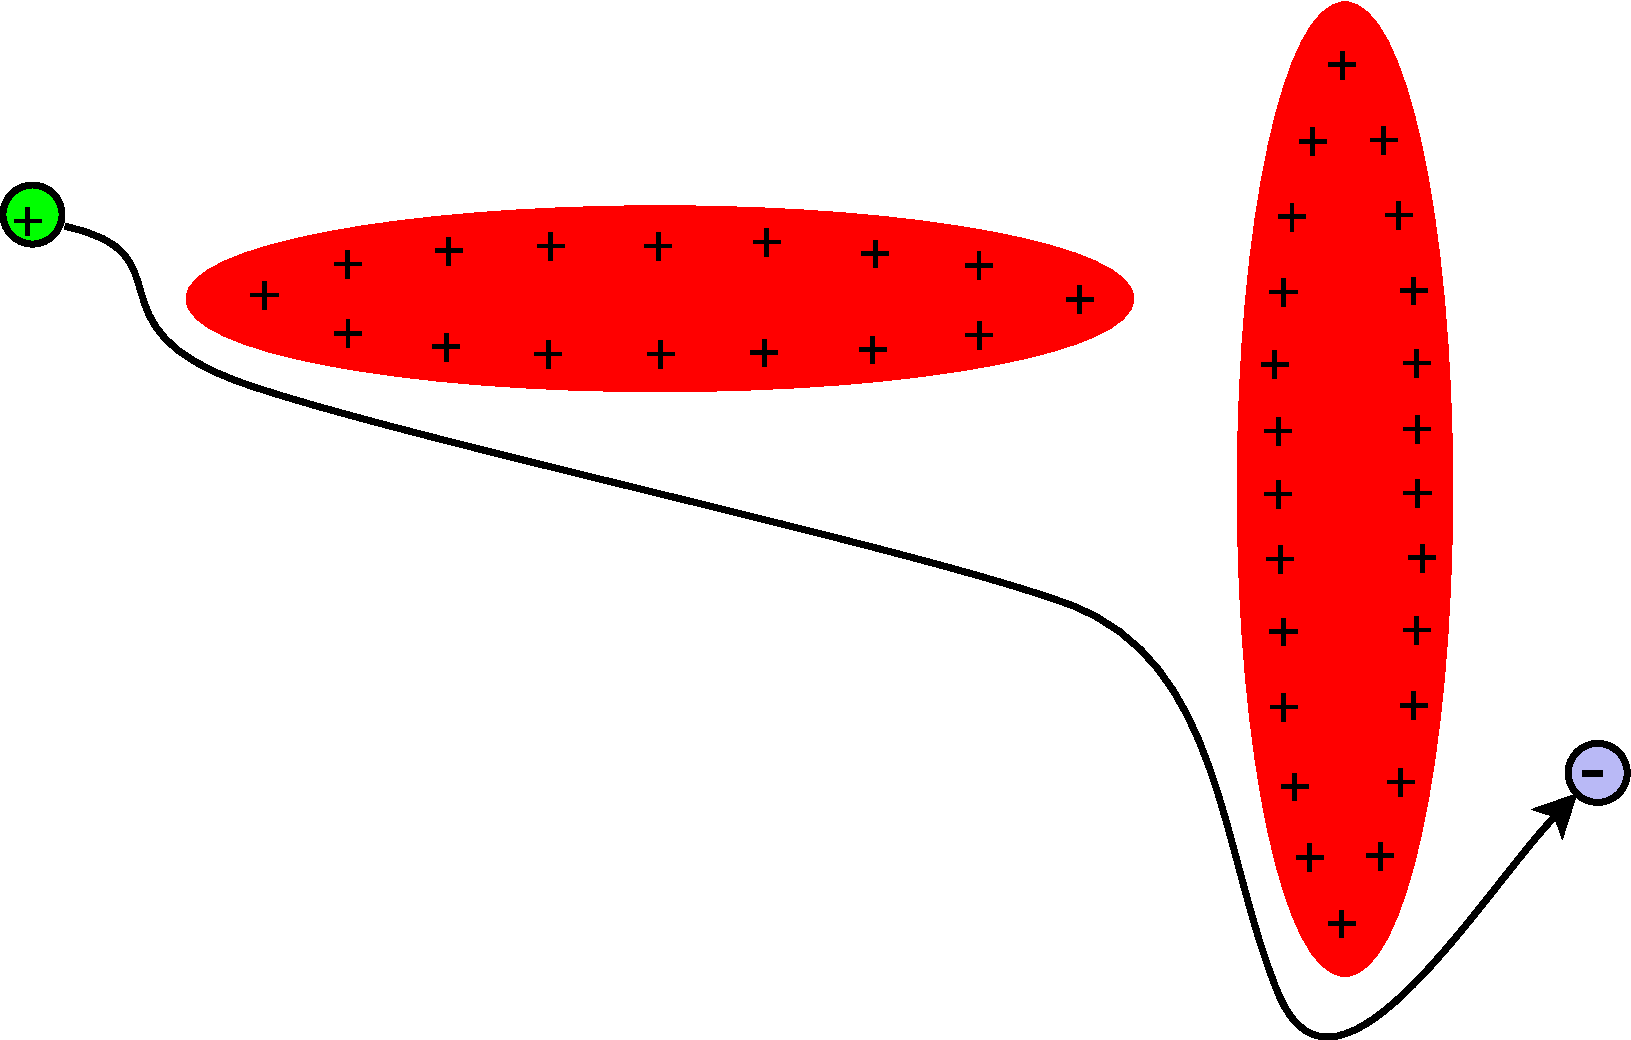
\includegraphics[width=0.4\textwidth,height=\textheight]{PlanningFigures/gradient_navigation.*}
\caption{Potential function navigation.}
\end{figure}

Vectors are seen as velocity not forces so this is a first order system.

The robot can move downhill using gradient descent:

\[\dot{c}(t) = -\nabla U(c(t)),\]

\[\displaystyle \frac{dx}{dt} = -\frac{\partial U}{\partial x}\]

\[\displaystyle \frac{dy}{dt} = -\frac{\partial U}{\partial y}\]

\(\nabla U(q)\), \(q_\text{start}\) Sequence
\(q_1, q_2, q_3, \dots , q_n\) \(q(0)=q_\text{start}\) \(i=0\)
\(q(i+1) = q(i) - \alpha (i) \nabla U(q(i))\) \(i++\)

It will stop when it reaches a critical point, \(q^*\):
\(\nabla U(q^*)=0.\) This point is a maximum, minimum or saddle point.
It depends on the eigenvalues of the \texttt{Hessian}

\[\begin{aligned}
H(U) = \begin{bmatrix}
          \displaystyle\frac{\partial^2 U}{\partial q_1^2} & \dots & \displaystyle\frac{\partial^2 U}{\partial q_1\partial q_n}\\[5mm]
          \displaystyle \vdots & \ddots & \vdots\\[5mm]
          \displaystyle\frac{\partial^2 U}{\partial q_n\partial q_1}  & \dots & \displaystyle\frac{\partial^2 U}{\partial q_n^2}\\[5mm]
         \end{bmatrix}
\end{aligned}\]

The Hessian is symmetric so the eigenvalues are real. Thus we get:

\begin{figure}
\centering
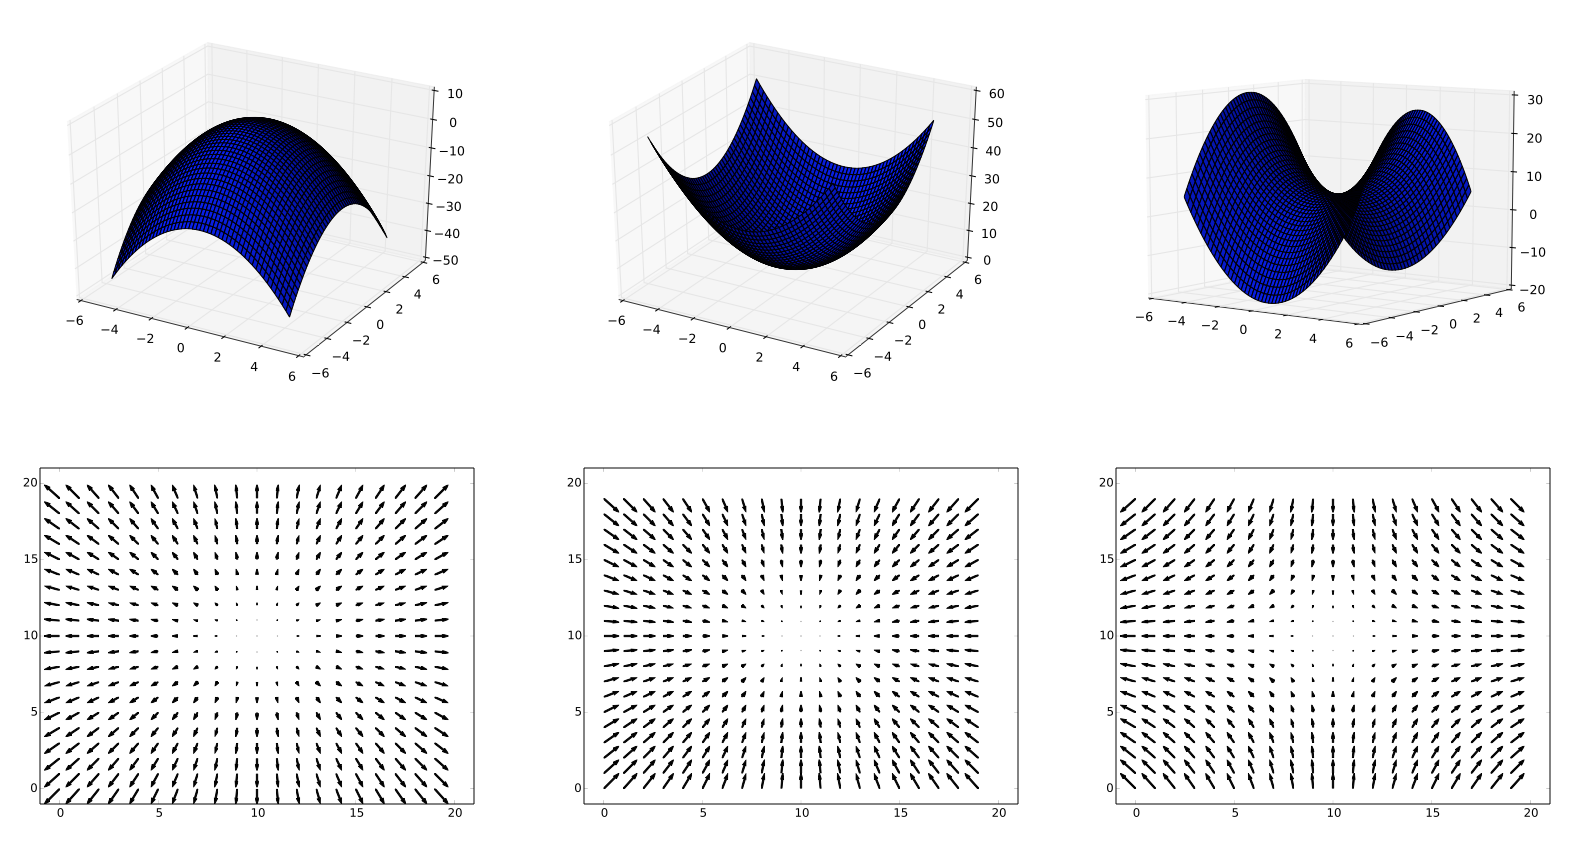
\includegraphics[width=0.9\textwidth,height=\textheight]{PlanningFigures/gradient_figures.png}
\caption{}
\end{figure}

\hypertarget{example-potential-functions}{%
\subsection{Example Potential
Functions}\label{example-potential-functions}}

Provide an example of an attractive potential function to the point
(5,6).

\[U_a = (x-5)^2 +(y-6)^2\]

The gradient can be found: \(\nabla U =<2x-10, 2y-12>\). Does
\(-\nabla U\) point to (5,6)? Pick a random point, (2,3). The vector
from (2,3) to (5,6) is \(<3,3>\). The negative of the gradient,
\(-\nabla U\) at (2,3) is \(<6,6>\) which is \(2<3,3>\) which works for
this point and is easy to show in general. The graph is shown in
\texttt{example2potential\_a}.

Next we write down a repulsive potential function for an ellipse. The
general equation of an ellipse is \((x-h)^2/a^2 + (y-k)^2/b^2 = 1\), and
for this example we will select \(a=1\), \(b=2\), \(h=3\), \(k=4\). A
repulsive function would be one that the gradient points away from.

An example of a repulsive potential:

\[U_r = \frac{1}{ (x-3)^2 + (y-4)^2/4 - 1}\]

The graph of this function is shown in \texttt{example2potential\_b}.

\begin{quote}
Attractive potential function.

Repulsive potential function.
\end{quote}

\hypertarget{constructing-potentials}{%
\subsection{Constructing Potentials}\label{constructing-potentials}}

As suggested above, we will construct the potential functions from two
basic types (\texttt{example2potential\_a},
\texttt{example2potential\_b}):

\begin{itemize}
\tightlist
\item
  \texttt{Attractive\ Potential}, denoted by \(U_\text{att}(q)\), and
\item
  \texttt{Repulsive\ Potentials}, denoted by \(U_\text{rep}(q)\).
\end{itemize}

The full potential function will then be a combination of the two basic
types. We will begin by just summing the potentials. This is the easiest
approach but as you will see does not scale to multiple objects
effectively. Using just addition, simple potential functions may be
constructed from these:

\[U(q) = U_\text{att}(q) + U_\text{rep}(q)\]

And more complicated functions may be constructed via

\[U(q) = U_\text{att}(q) + \sum_i U_{\text{rep}\, i}(q)\]

We also assume that the outer boundary is not critical and so we ignore
outer boundary effects. Later we will be able to include the boundary.

\textbf{Attractive Potential} A very simple function to use for the
attractive potential is

\[U_\text{att} = k_0\left[(x-x_0)^2 + (y-y_0)^2\right]\]

where \((x_0, y_0)\) is the location of the goal. The value \(k_0\)
selects how steep the function walls are and thus changes the magnitude
of the resulting gradient. This is the force pushing the object to the
goal. We will balance \(k_0\) with the constants of the other functions
to gain an effective potential function surface. See
\texttt{example2potential\_a}.

\textbf{Repulsive Potential} A single repulsive potential can be formed
by modifying the attractive potential. Assume that you can enclose the
obstacle in a circle \((x-x_0)^2 + (y-y_0)^2 = r^2\) for some radius
\(r\) and some center \((x_0,y_0)\). Let

\[\rho = (x-x_0)^2 + (y-y_0)^2 - r^2\]

The function \(\rho\) is zero on the boundary of the circle and is
positive outside the circle. It is a paraboloid that opens up. Then the
repulsive potential is can be formed from \(\gamma/\rho\) or

\[U_\text{rep} = \frac{\gamma}{(x-x_0)^2 + (y-y_0)^2 - r^2}\]

\(U_\text{rep}\) is a function that goes to infinity at you approach the
circle. See \texttt{example2potential\_b}. The term \(\gamma\) is the
strength of the field. It is a parameter which can be varied to adjust
the relative force exerted by the repulsive field. It can shape the
robot path an sometimes avoid local extremals.

Some authors like to shut down the repulsive potential by subtracting
off a constant so it is zero outside a larger circle:

\[\begin{aligned}
U_\text{rep} = \left\{
\begin{array}{ll}
\displaystyle \frac{\gamma}{(x-x_0)^2 + (y-y_0)^2 - r^2} - \sigma & \text{for  } \rho < \frac{\gamma}{\sigma}\\[3mm]
0 &  \text{for  } \rho \geq \frac{\gamma}{\sigma}.
\end{array} \right.
\end{aligned}\]

Because there are quadratic functions involved, the growth can
excessive. One way to deal with large values is to use conic potentials
instead of quadratic potentials. Let \(q=(x,y)\) and
\(q_\text{goal} = (x,y)_\text{goal}\). The conic potential:

\[U_\text{att} = \gamma d(q, q_\text{goal})\]

The gradient is then

\[\nabla U(q) = \frac{\gamma}{d(q, q_\text{goal})} (q-q_\text{goal})\]

This presents numerical issues due to the discontinuity, so normally one
uses \(U(q) = \gamma d^2(q, q_\text{goal})\)

\[\nabla U(q) = \gamma (q-q_\text{goal})\]

Velocity is too large far away and will overwhelm other fields. We use a
linear velocity for far field and quadratic velocity for near field. The
switch over point is at distance \(d^*_\text{goal}\):

\[\begin{aligned}
U_\text{att}(q) = \left\{ \begin{array}{ll} (1/2)\gamma d^2(q, q_\text{goal}), & d(q, q_\text{goal})\leq d^*_\text{goal},\\[3mm]
d^*_\text{goal}\gamma d(q, q_\text{goal}) - (1/2)\gamma (d^*_\text{goal})^2, & d(q, q_\text{goal})> d^*_\text{goal},
\end{array}\right.
\end{aligned}\]

which gives

\[\begin{aligned}
\nabla U_\text{att}(q) = \left\{ \begin{array}{ll} \gamma (q -q_\text{goal}), & d(q, q_\text{goal})\leq d^*_\text{goal},\\[3mm]
d^*_\text{goal}\gamma \frac{(q -q_\text{goal})}{d(q, q_\text{goal})}, & d(q, q_\text{goal})> d^*_\text{goal},
\end{array}\right.
\end{aligned}\]

The repulsive potential is the same as the one above. We rewrite the
expression in slightly different notation where the \(\gamma/\sigma\)
term is replaced by \(1/Q^*\) which is a measure of distance away from
the obstacle boundary. Essentially \(Q^*\) is the cutoff distance for
when we no longer express the repulsive potential field. The formula in
the new notation is

\[\begin{aligned}
U_\text{rep}(q) = \left\{ \begin{array}{ll} (1/2)\eta \left( \frac{1}{D(q)} - \frac{1}{Q^*}\right) , &
D(q) \leq Q^*,\\[3mm]
0, & D(q) > Q^*
\end{array}\right.
\end{aligned}\]

This becomes a very complicated formula when the obstacles are no longer
circles. It is very difficult to arrive at a formula for the closest
obstacle. Finding equidistance lines is a whole issue alone. We will
address this when we discuss Voronoi decomposition.

Note that placing repulsive potentials in can change the location of the
minimum that you have setup through the attractive potential. This is
one reason we go to the trouble of placing a cutoff on the obstacle
potentials. A simple one dimensional example can demonstrate. Assume you
want your minimum to be at \(x=0\), so you try \(U_a = x^2\). Next you
place in a repulsive potential at \(x=5\), \(U_r = |x - 5|^{-1}\).
Combining we have

\[U = x^2 + \frac{1}{|x - 5|}.\]

Compute the derivative and set to zero:

\[\frac{dU}{dx} = 2x - \frac{\mbox{sign}(x-5)}{|x - 5|^2} = 0.\]

For \(x<5\) we have

\[\frac{dU}{dx} = 2x - \frac{1.0}{|x - 5|^2} = 0\]

which can solved: \(2x(x-5)^2 = 1\) or \(x\approx 0.02\). No longer at
\(x=0\).

\textbf{Summary:}

\[U(q) = U_\text{att}(q) + U_\text{rep}(q)\]

\[\begin{aligned}
U_\text{att}(q) = \left\{ \begin{array}{ll} (1/2)\gamma d^2(q, q_\text{goal}), & d(q, q_\text{goal})\leq d^*_\text{goal},\\[3mm]
d^*_\text{goal}\gamma d(q, q_\text{goal}) - (1/2)\gamma (d^*_\text{goal})^2, & d(q, q_\text{goal})> d^*_\text{goal},
\end{array}\right.
\end{aligned}\]

\[\begin{aligned}
U_\text{rep}(q) = \left\{ \begin{array}{ll} (1/2)\eta \left( \frac{1}{D(q)} - \frac{1}{Q^*}\right) , &
D(q) \leq Q^*,\\[3mm]
0, & D(q) > Q^*
\end{array}\right.
\end{aligned}\]

The distance \(D(q)\) can be determined from a LIDAR sweep if the robot
is located at \(q\).

\begin{figure}
\centering
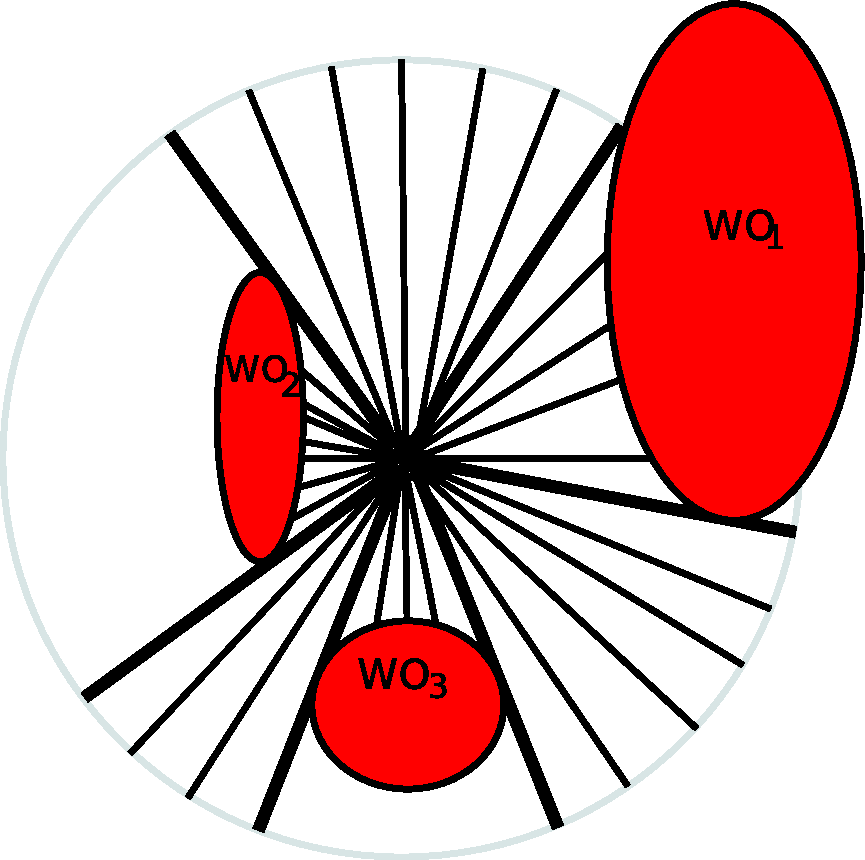
\includegraphics[width=0.35\textwidth,height=\textheight]{PlanningFigures/range.*}
\caption{LIDAR Range map.}
\end{figure}

To compute the potential function, you need to know all of the
distances, not just from a single point \(q\).

Often the environment is represented on a grid which can simplify the
planning process in some cases. Our first step is to remove the analytic
repulsive potential and replace it with a discrete method known as the
Brushfire algorithm. This can remove the problems related to finding
repulsive potentials that don't overwhelm the attractive potential.

\[U = (x-5)^2 +(y-6)^2 +  \frac{\gamma}{ (x-3)^2 + (y-4)^2/4 - 1}\]

\begin{figure}
\centering
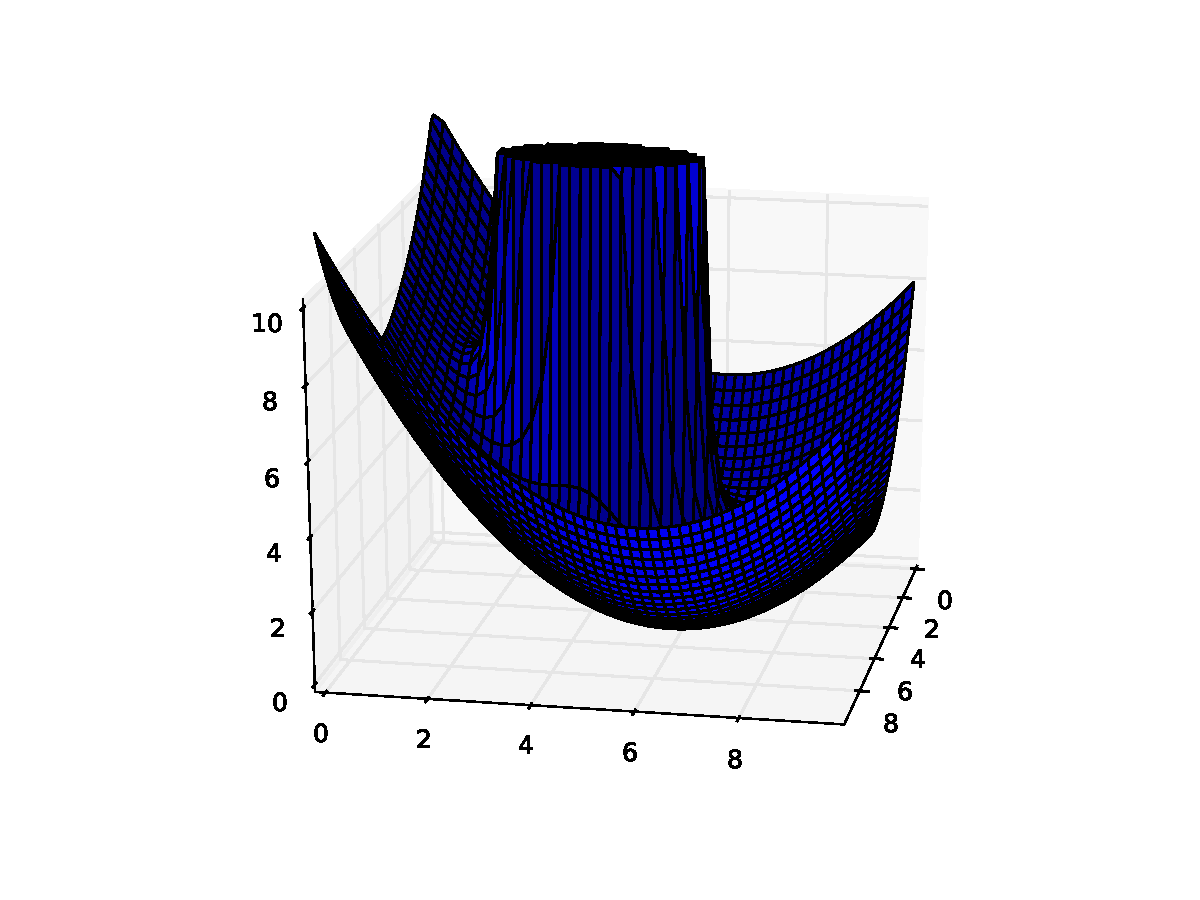
\includegraphics[width=0.5\textwidth,height=\textheight]{PlanningFigures/potential3.*}
\caption{}
\end{figure}

The equations of motion that generate the path are

\[\begin{aligned}
\begin{array}{l}
\displaystyle \frac{dx}{dt} = -\frac{\partial U}{\partial x} = -2(x-5) + \frac{2\gamma(x-3)}{[(x-3)^2 + (y-4)^2/4 - 1]^{2}}\\[10pt]
\displaystyle \frac{dy}{dt} = -\frac{\partial U}{\partial y} = -2(y-6) + \frac{\gamma(y-4)/2}{[(x-3)^2 + (y-4)^2/4 - 1]^{2}}
\end{array}
\end{aligned}\]

This is solved by using a discrete approach which is known as steepest
descents.

\[\begin{aligned}
\begin{array}{l}
\displaystyle x_{n+1} = x_n  - \eta\left\{2(x_n-5) - \frac{2\gamma(x_n-3)}{[(x_n-3)^2 + (y_n-4)^2/4 - 1]^{2}}\right\}\\[10pt]
\displaystyle y_{n+1} = y_n -   \eta\left\{2(y_n-6) - \frac{\gamma(y_n-4)/2}{[(x_n-3)^2 + (y_n-4)^2/4 - 1]^{2}}\right\}
\end{array}
\end{aligned}\]

Note that \(\gamma\) is a measure of field strength and \(\eta\) is a
step size parameter. Moving these two around is useful to adjust for
better computed paths.

\begin{verbatim}
import numpy as np
import scipy as sp
import pylab as plt
from matplotlib.patches import Ellipse

NP = 200
t = np.arange(0,NP,1)
x = np.zeros((NP))
y = np.zeros((NP))
x[0] = 0.0
y[0] = 0.0
gamma = 1.0
zeta = 0.1

for i in range(1,NP):
  v = gamma/(((x[i-1]-3.0)**2 + ((y[i-1]-4.0)**2)/4 -1.0)**2)
  vx = 2.0*(x[i-1]-5.0) - 2*(x[i-1]-3)*v
  vy = 2.0*(y[i-1]-6.0) - 0.5*(y[i-1]-4)*v
  vn = np.sqrt(vx*vx+vy*vy)
  vx2 = vx/vn
  vy2 = vy/vn
  print v, -vx2, -vy2
  x[i] = x[i-1] - zeta*vx2
  y[i] = y[i-1] - zeta*vy2

ell = Ellipse((3.0,4.0),2,4,0)
a = plt.subplot(111, aspect='equal')
ell.set_alpha(0.1)
a.add_artist(ell)

plt.plot(x,y, 'b.')
plt.xlabel('X')
plt.ylabel('Y')
plt.title('Path')
plt.show()
\end{verbatim}

\begin{figure}
\centering
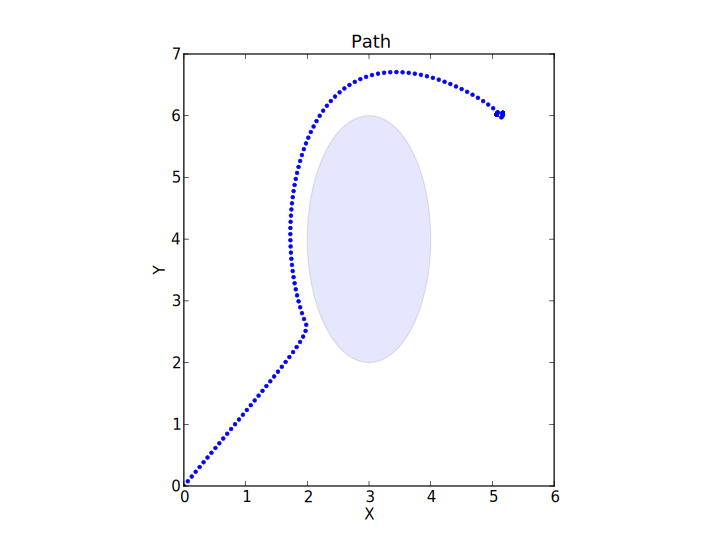
\includegraphics[width=0.85\textwidth,height=\textheight]{PlanningFigures/potentialavoid1a.*}
\caption{}
\end{figure}

Let the domain be the square \(0\leq x \leq 10\), \(0\leq y \leq 10\).

\begin{itemize}
\tightlist
\item
  Place the start position at (1,1)
\item
  Place the goal position at (9,8)
\item
  Obstacle 1: disk centered at (4,3) of radius 2.5.
\item
  Obstacle 2: disk centered at (7,8) of radius 1.
\end{itemize}

What is the potential function?

Obstacles in red...

\begin{figure}
\centering
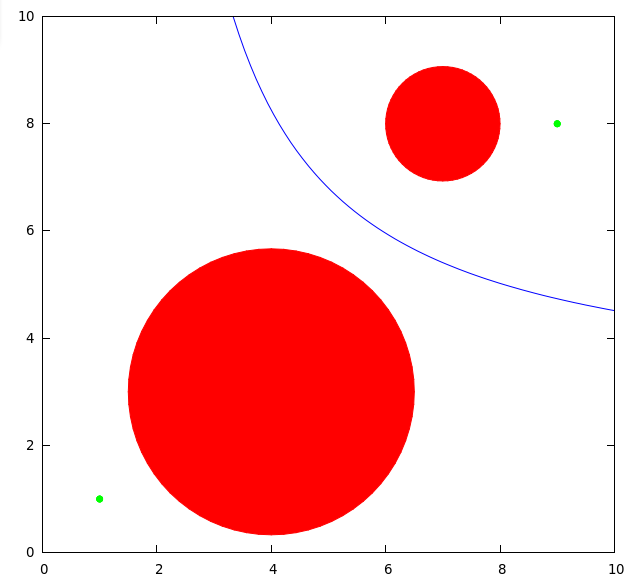
\includegraphics[width=0.5\textwidth,height=\textheight]{PlanningFigures/circles.png}
\caption{Two obstacles and the resulting equal distance line.}
\end{figure}

What is the attractive potential? Let \(q = (x,y)\),

\[U_a(q) =(x -9)^2 + (y -8)^2.\]

What is the repulsive potential?

\[U_r (q)= \frac{\gamma_1}{(x-4)^2 + (y-3)^2 - 2.5^2} + \frac{\gamma_2}{(x-7)^2 + (y-8)^2 - 1^2}\]

The resulting potential is the sum:

\[U = U_a(q) + U_r (q)= (x -9)^2 + (y -8)^2 +\]

\[\frac{\gamma_1}{(x-4)^2 + (y-3)^2 - 2.5^2} + \frac{\gamma_2}{(x-7)^2 + (y-8)^2 - 1^2}\]

\begin{figure}
\centering
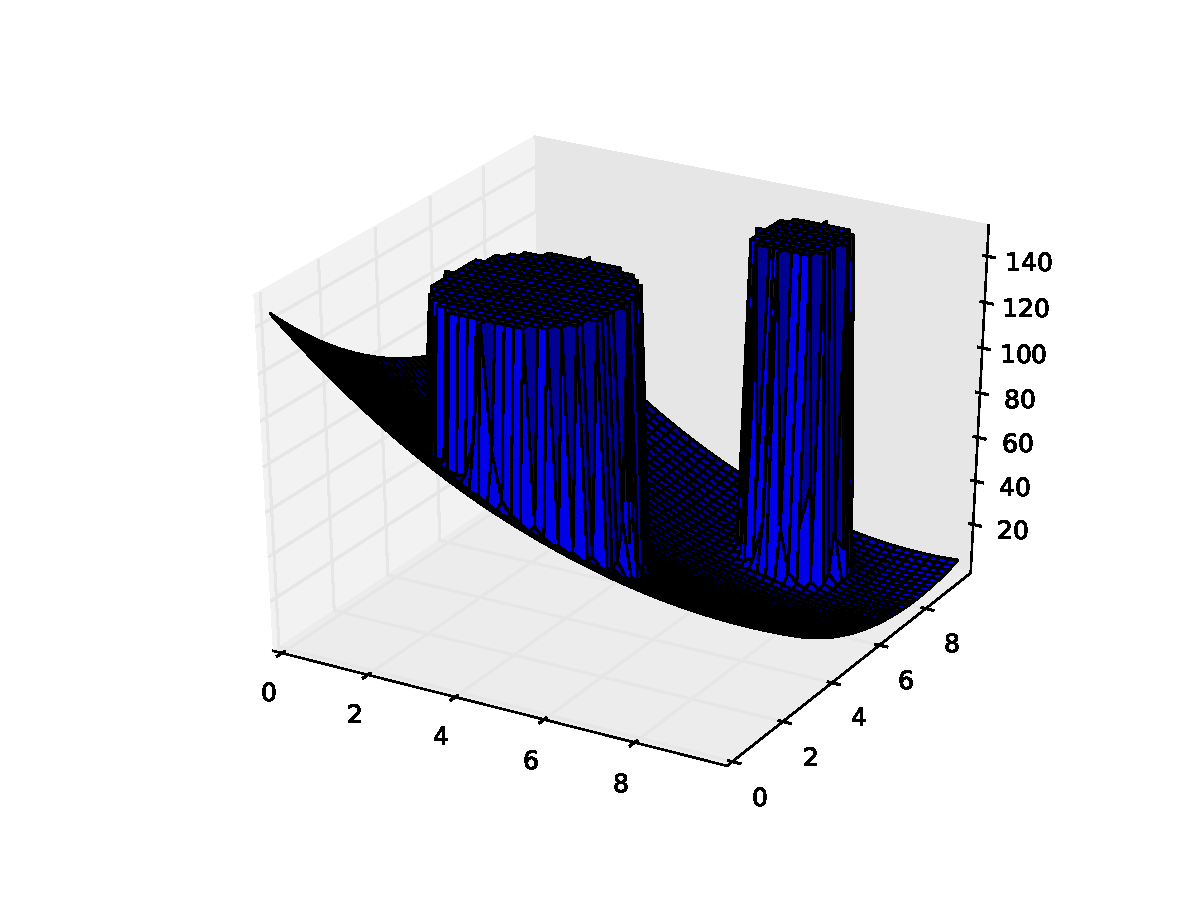
\includegraphics[width=0.7\textwidth,height=\textheight]{PlanningFigures/potential4.*}
\caption{Potential function surface.}
\end{figure}

Resulting navigation.

These simple functions work well for simple domains. However, when the
obstacles increase, then the simple potentials cease to be effective. A
more methodical approach is needed.

If you looked carefully at the path in \texttt{fig:Resultingnavigation},
you will notice that the path appears to oscillate when it gets near the
large obstacle. Indeed this is what is happening. This oscillation is a
direct result of the steepest descent algorithm is appears in many
numerical optimization routines. The numerics will follow the steepest
gradient and will oscillate back and forth along the steep walls. It
will slowly average out traversing the mean path which will trace the
valley floor, \texttt{fig:numericaloscillation}.

\begin{quote}
Numerical Oscillation near steep gradients.
\end{quote}

There is nothing particularly special regarding the functions we have
presented. Our goal is to find a potential surface which can ``navigate"
a vehicle from start to finish. Getting familiar with the shapes and
level sets of graphs can be very helpful. This can help one in the
construction process. Typically we want our level set to track an
obstacle boundary.

Construct a function which directs the craft onto the line
\(y = 2x + 3\). Then \(U = (2x+3-y)^2\) will suffice. This function has
a minimum along \(y = 2x + 3\) and increases as you move away from the
line.

Keep in mind that you must be very careful combining the functions since
they can interact in very complex ways. You may have to have cutoff
distances from obstacles to keep them from corrupting each other.

\hypertarget{higher-dimensions}{%
\subsection{Higher Dimensions}\label{higher-dimensions}}

One of the advantages of potential functions is that they scale to
higher dimensions in a very efficient manner. We will start with three
dimensions. The attractive and repulsive potentials follow the same
pattern as we saw in two dimensions.

Construct an attractive potential for the the point \(x_0,y_0,z_0\).

\[U_{att} = (x-x_0)^2 + (y-y_0)^2 + (z-z_0)^2,\]

and

\[\nabla U_{att} = \langle 2(x-x_0) , 2(y-y_0) , 2(z-z_0)\rangle\]

Construct a repulsive potential for a spherical obstacle centered
\(x_0,y_0,z_0\) of radius \(R\).

\[U_{rep} = \displaystyle \frac{\gamma}{(x-x_0)^2 + (y-y_0)^2 + (z-z_0)^2 - R^2}\]

and

\[\nabla U_{rep} = \displaystyle \frac{-2\gamma \langle (x-x_0) , (y-y_0) ,  (z-z_0)\rangle}{\left( (x-x_0)^2 + (y-y_0)^2 + (z-z_0)^2 - R^2\right)^2}\]

Build a function that can direct a drone to a landing pad. Assume the
landing pad is at (0,0,0). We construct a cone centered at the landing
pad which will ``pull" the drone in. We can take a simple attractive
function

\[U_{att} =  x^2 + y^2  + \alpha z^2 = r^2 + \alpha z^2, \quad r = \sqrt{x^2 + y^2}\]

and then a vertical squeeze function

\[U_{att2} = (z -r)^2.\]

The resulting potential is \(U = U_{att}  + \gamma U_{att2}\),

\[U = r^2 + \alpha z^2 +\gamma (z -r)^2  =  (1+\gamma)r^2 + (\gamma + \alpha) z^2 - 2\gamma rz\]

\[= (1+\gamma)(x^2 + y^2) + (\gamma + \alpha) z^2 - 2\gamma z\sqrt{x^2 + y^2}.\]

For the attractive function, the parameter \(\alpha\) can be used to
vary the relative strength in the \(z\) direction. In the squeeze
function, the parameter \(\gamma\) can be used to adjust the strength of
that field component.
